\renewcommand{\theequation}{\theenumi}
\begin{enumerate}[label=\arabic*.,ref=\thesubsection.\theenumi]
\begin{figure}[!h]
\centering
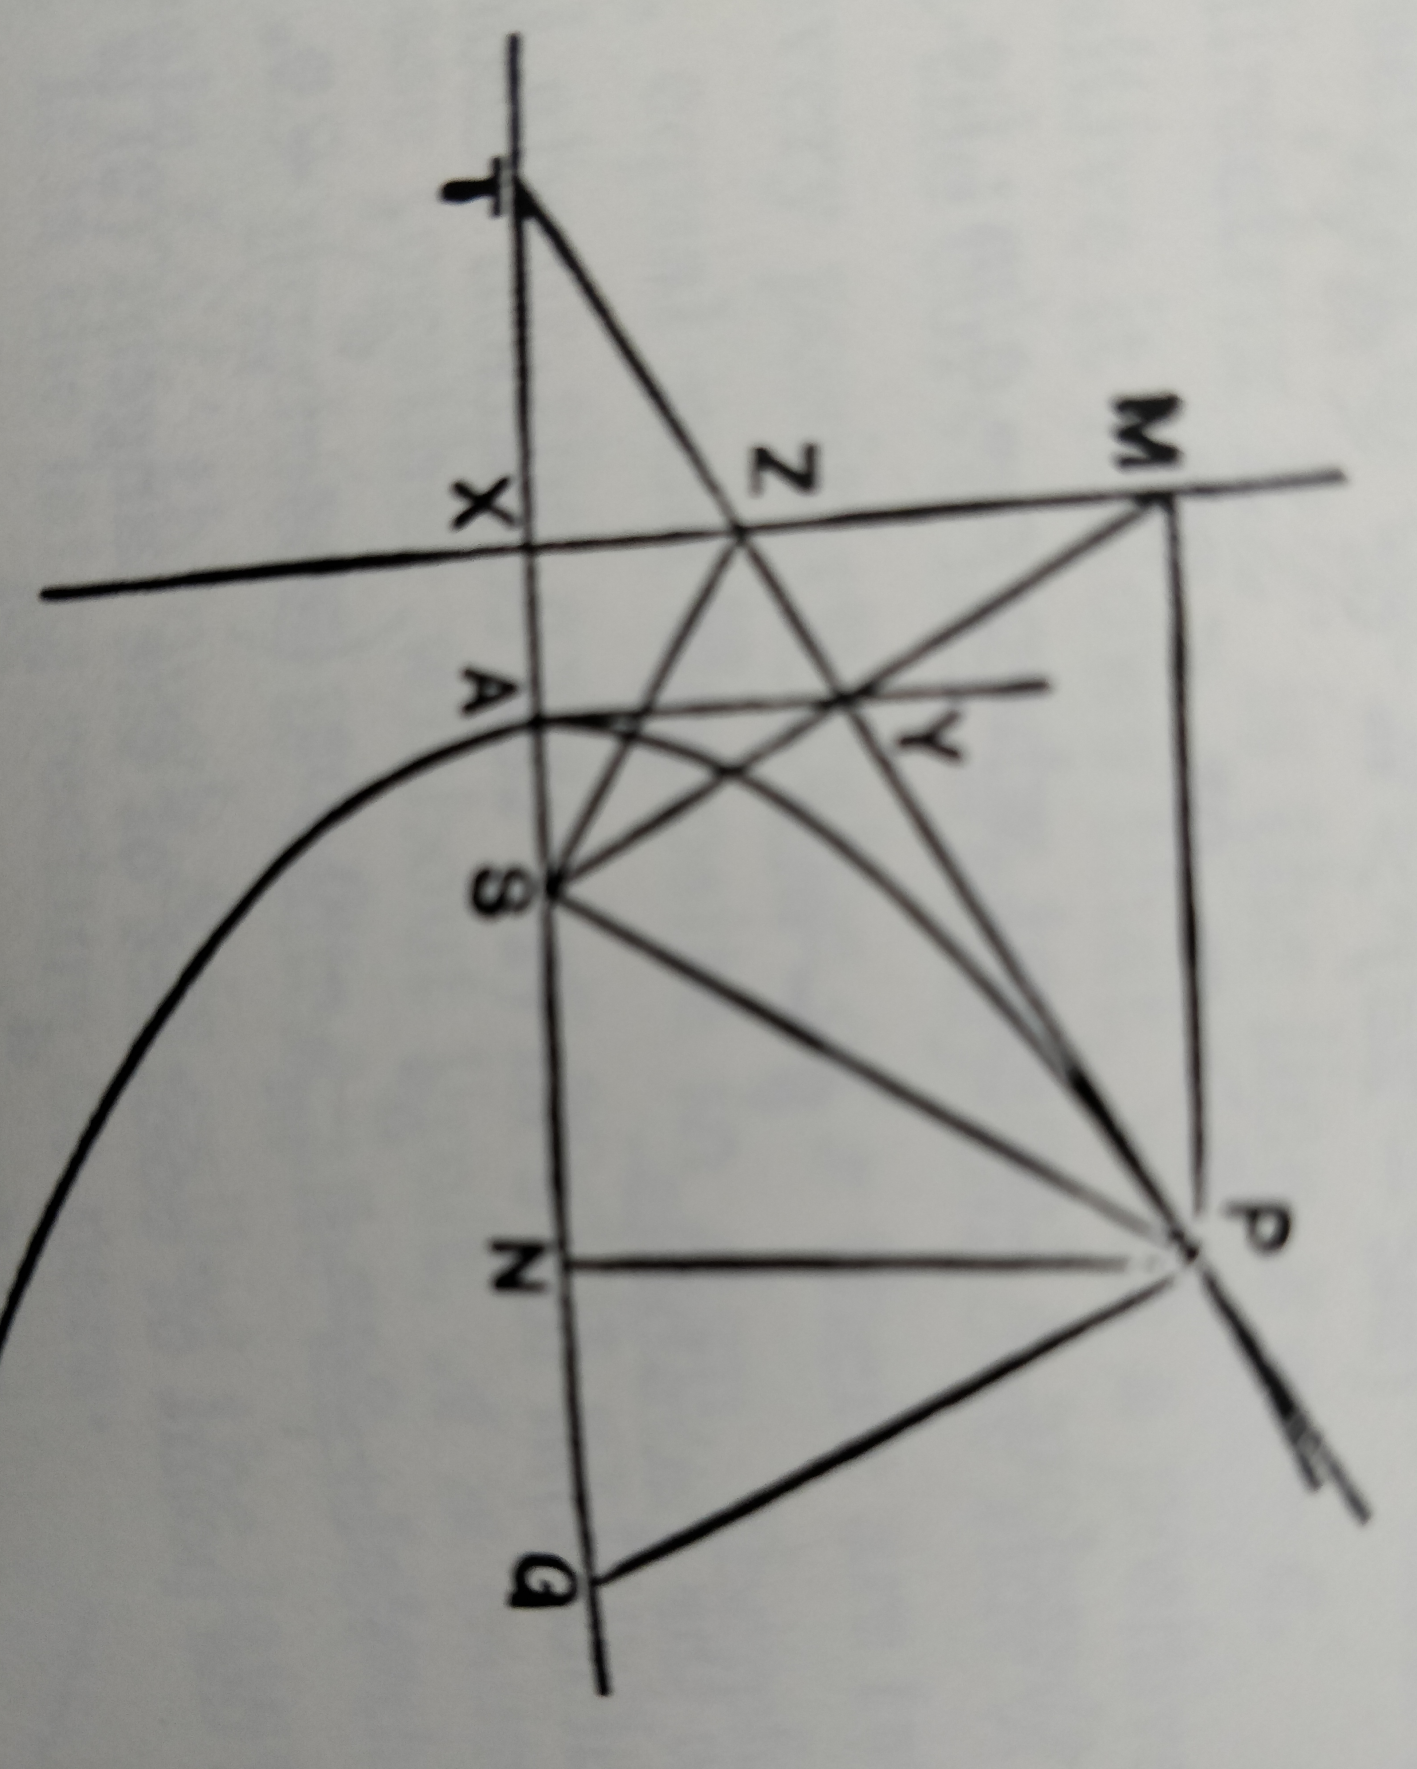
\includegraphics[angle=90,origin=c,width=\columnwidth]{./figs/parabola.eps}
\caption{}
\label{fig:parabola}
\end{figure}
%\begin{enumerate}[1.]
\numberwithin{equation}{enumi}
\item Show that the line 
\begin{align}
\myvec{4 & -2}\vec{x} + a= 0
\end{align}
touches the parabola 
\begin{align}
\vec{x}^T\myvec{0 & 0\\0 & 1}\vec{x}-4a\myvec{1 & 0 }\vec{x}= 0 
\end{align}
and find the coordinates of
the point of contact.
\item Find the point of intersection of the parabolas 
\begin{align}
\vec{x}^T\myvec{0 & 0\\0 & 1}\vec{x}-4a\myvec{1 & 0 }\vec{x}= 0 
\\
\vec{x}^T\myvec{1 & 0\\0 & 0}\vec{x}-4a\myvec{0 & 1 }\vec{x}= 0 
\end{align}
other than the origin, and prove that the tangents
at this point are inclined at an angle $\tan^{-1}\frac{3}{4}$.
\item Find the points in which the line 
\begin{align}
\myvec{8 & -1}\vec{x} = a
\end{align}
 cuts the parabola 
\begin{align}
\vec{x}^T\myvec{0 & 0\\0 & 1}\vec{x}-4a\myvec{1 & 0 }\vec{x}= 0 
\end{align}
and find the point where
the tangents at these points intersect.
\renewcommand{\theequation}{\theenumi}
\item A line through the vertex $\vec{A}$ of the parabola 
\begin{align}
\vec{x}^T\myvec{0 & 0\\0 & 1}\vec{x}-4a\myvec{1 & 0 }\vec{x}= 0 
\end{align}
makes an angle of $60\degree$ with
the axis and cuts the curve again in $\vec{P}$.  Find the equation of the tangent at $\vec{P}$,
and show that the area of the triangle this tangent makes with the axes is $\frac{4a^2}{3\sqrt{3}}$.
\item Prove that in  Fig. \ref{fig:parabola}
\begin{equation}
SG=SP
\end{equation}
\item Prove that $t_1t_2=-1$ is the condition that the chord joining the points with parameters $t_1, t_2$ on
a parabola shall pass through the focus.
\item Prove that the tangents drawn to a parabola from a point on the
directrix are at right angles and that their chord of contact passes
through the focus.
\item If in Fig. \ref{fig:parabola} $PS$ cuts the curve again in $\vec{Q}$, prove that $QA$ passes
through $\vec{M}$.
\item Through the vertex $\vec{A}$ of a parabola chords $AP$, $AP$ at right angles
to one another are drawn.  Prove that $PA$ cuts the axis in a fixed point.
\item Find the coordinates of the other point in which the normal at $\myvec{at^2\\2at}$
meets the parabola 
\begin{align}
\vec{x}^T\myvec{0 & 0\\0 & 1}\vec{x}-4a\myvec{1 & 0 }\vec{x}= 0 
\end{align}
;
 and prove that two normal chords that cut at right angles
divide one another in the ratio $1:3$.
\item Three normals are drawn to a parabola from the point $\myvec{h\\k}$.  Prove that
the centroid of the triangle formed by their feet is the point $\myvec{\frac{2}{3}\brak{h-2a}\\0}$.\numberwithin{equation}{enumi}
\item Find the equation of the tangent to the parabola 
\begin{align}
\vec{x}^T\myvec{0 & 0\\0 & 1}\vec{x}-4a\myvec{1 & 0 }\vec{x}= 0 
\end{align}
%
 that is parallel
to the normal at $\vec{P}= \myvec{at^2\\2at}$; and prove that, if this tangent meets the axis in $T$
and $PN$ is the ordinate of $P$ and $A$ is the vertex, then
\begin{equation}
TA.AN=a^2
\end{equation}
\item Prove that the circle 
\begin{align}
\vec{x}^T\vec{x}+2\myvec{g & f }\vec{x}+c= 0 
\end{align}
%
 cuts the parabola 
\begin{align}
\vec{x}^T\myvec{0 & 0\\0 & 1}\vec{x}-4a\myvec{1 & 0 }\vec{x}= 0 
\end{align}

 in four points the sum of
whose ordinates is zero; and conversely that if four ponits on a parabola be
such that the sum of their ordinates is zero then the four points lie on a circle.
\item Prove that the orthocentre of a triangle whose sides all touch a parabola
lies on the directrix.
\item A chord $POQ$ of a parabola 
\begin{align}
\vec{x}^T\myvec{0 & 0\\0 & 1}\vec{x}-4a\myvec{1 & 0 }\vec{x}= 0 
\end{align}

 cuts the axis in a fixed point $\vec{O}$.  $PN$, $QM$ are the ordinates of $\vec{P}$ and $\vec{Q}$,
and $\vec{A}$ is the vertex.  Prove that
\begin{align}
NP.MQ+4a.AO=0
\end{align}
\item From a point $\vec{P}= \myvec{at_1^2\\2at_1}$ on the parabola 
\begin{align}
\vec{x}^T\myvec{0 & 0\\0 & 1}\vec{x}-4a\myvec{1 & 0 }\vec{x}= 0 
\end{align}
 two chords $PQ$, $PR$ are drawn normal to the curve at $\vec{Q}$
and $\vec{R}$.  Prove that, if $\vec{Q}$, $\vec{R}$ are the points with parameters $t_2$, $t_3$ on the curve, then $t_2t_3=2$, and the equation
of $QR$ is
\begin{align}
\myvec{2 & t_1}\vec{x} + 4a= 0
\end{align}
\item Prove that the normals to a parabola at the ends of a chord whose inclination to the axis is $\theta$ meet on the
normal whose inclination is $\tan^{-1}\brak{2\cot\theta}$.
\item Prove that, if two parabolas are on the same side of the same directrix and have their axes in the same line, then they intersect
at a distance from the directrix equal to one-quarter of the sum of their latera recta.

\end{enumerate}
